\documentclass[10pt]{article}

\usepackage{graphicx}
\usepackage{graphics}
\usepackage{multicol}
\usepackage{epsfig,amsmath,amsfonts}

\makeatletter                                   % Make '@' accessible. 
\oddsidemargin=0in                              % Left margin minus 1 inch.
\evensidemargin=0in                             % Same for even-numbered pages.
\marginparsep=0pt                               % Space between margin & text

\renewcommand{\baselinestretch}{1}              % Double spacing

\textwidth=6.5in                                % Text width (8.5in - margins).
\textheight=9in                                 % Body height (incl. footnotes)

\topmargin=0in                                  % Top margin minus 1 inch.
\headsep=0.0in                                  % Distance from header to body.
\skip\footins=4ex                               % Space above first footnote.
\hbadness=10000                                 % No "underfull hbox" messages.
\makeatother                                    % Make '@' special again.


\begin{document}

\fontfamily{cmss}                               % Make text sans serif.
\fontseries{m}                                  % Medium spacing.
\fontshape{n}                                   % Normal: not bold, etc.
\fontsize{10}{10}                               % 10pt font, 10pt line spacing 

\title{Ad-Hoc Routing Component Architecture}
\author{Philip Levis}
\maketitle

\fontfamily{cmr}                                % Make text Roman (serif).
\fontseries{m}                                  % Medium spacing.
\fontshape{n}                                   % Normal: not bold, etc.
\fontsize{10}{10}                               % 10pt font, 10pt line spacing


\begin{figure}
\centering
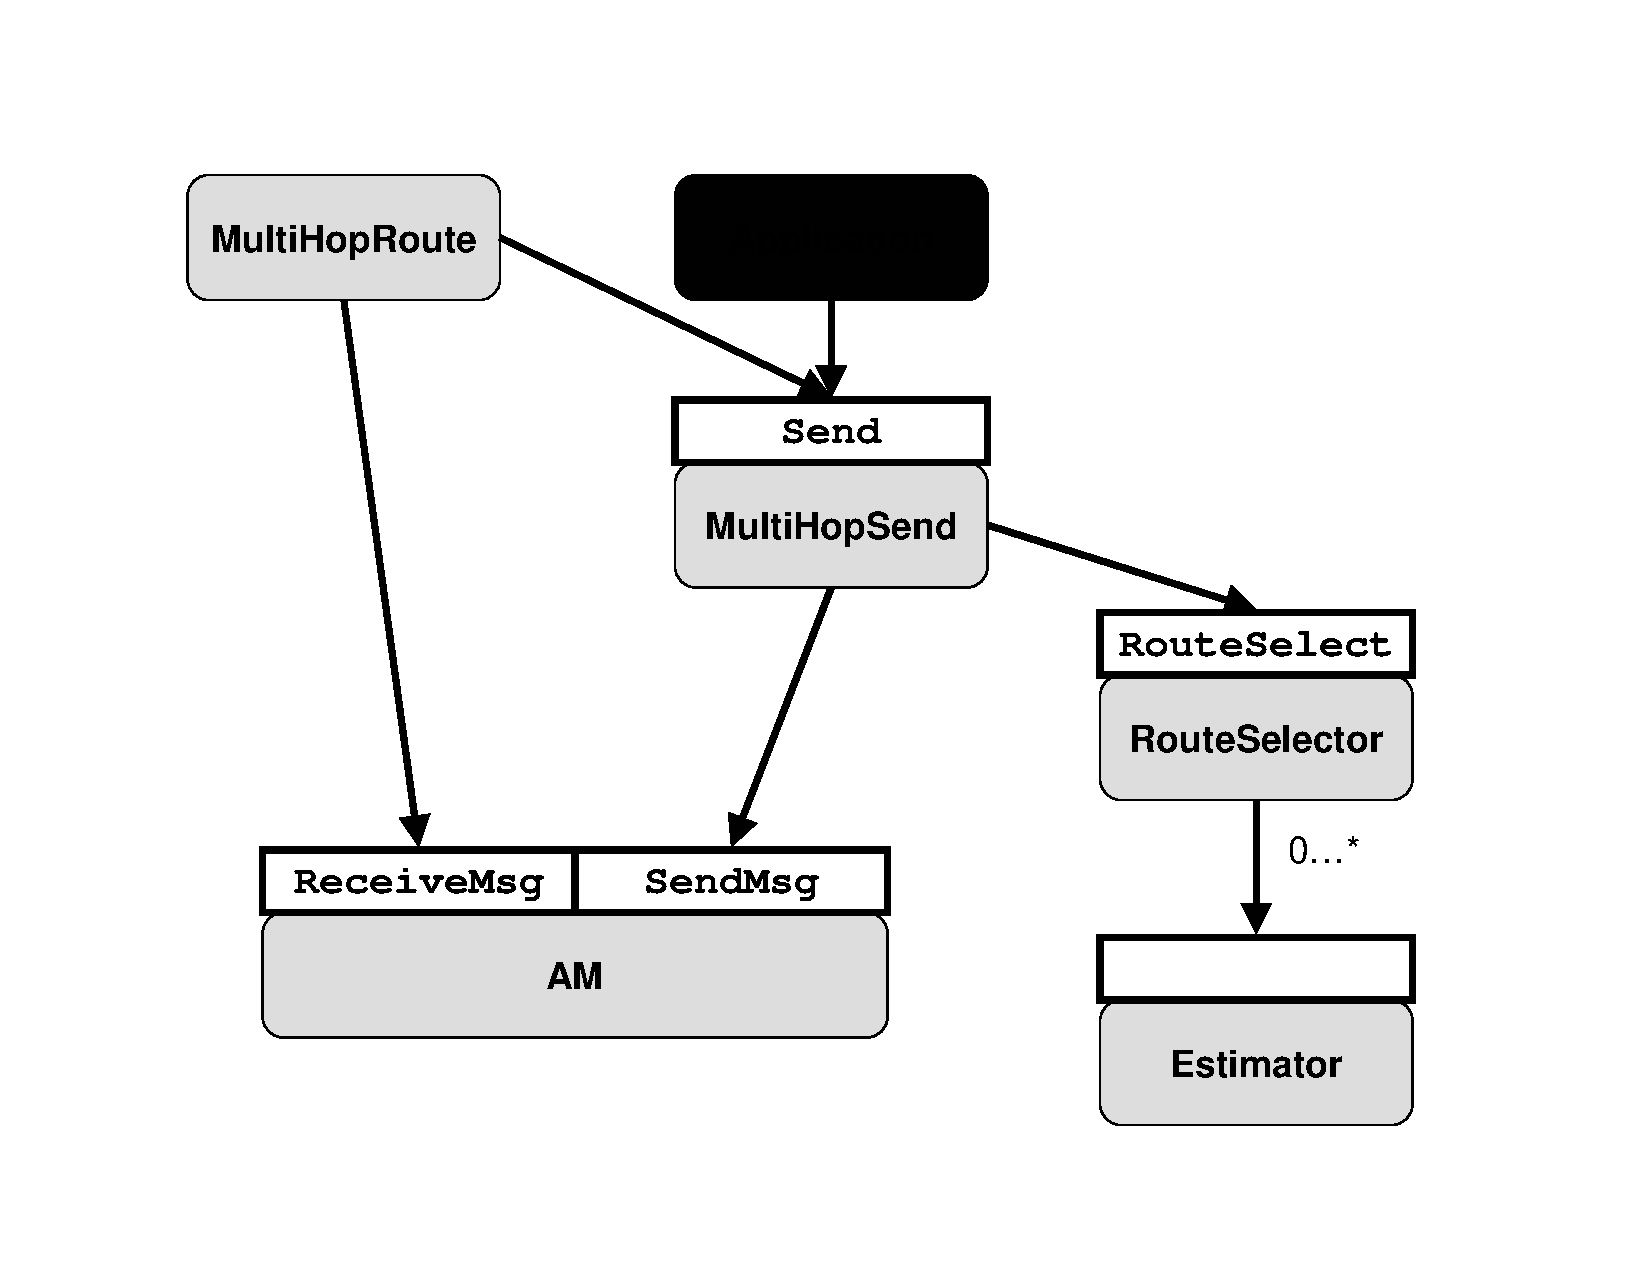
\includegraphics[angle=-90,scale=.25]{fig/arch.pdf}
\caption{Component Architecture}
\label{fig:arch}
\end{figure}


\section*{Introduction}

TinyOS has a pressing need for a good ad-hoc routing service. Several
protocols have been developed, each of which has acknowledged
problems. One issue that has arisen is separating policies from
mechanisms; it would be a great help to have the ability to easily
experiment with a variety of different algorithmic building blocks,
each of which can be easily interchanged. We have therefore developed
a general ad-hoc protocol component architecture; algorithms should be
built in components that follow this architecture, so that they can be
easily incorporated into different combinations for testing and
evaluation.

\section*{Overview}


Multi-hop routing has been broken into several components, shown in
Figure \ref{fig:arch}. The black box at the top of the figure is the
application, which only makes calls on the MultiHopSend component
(probably through a MultiHop configuration). The MultiHopRoute
component also uses MultiHopSend to forward packets. MultiHopSend is
responsible for decisions such as whether to retransmit or to try
another route.

Actual route selection is performed by the RouteSelector component
through the RouteSelect interface. MultiHopSend, while aware of the
size of the protocol headers, never interacts with them; instead, it
merely passes buffers to RouteSelect for the values to be filled in.

RouteSelector depends on some number of Estimator components to make
decisions on which route to use. For example, a min-hop algorithm
(similar to BLESS or Narpro) might have an estimator that listens for
protocol messages and updates routing tables accordingly. A network
link quality estimator might use link quality broadcasts to
communicate with neighbors. A given RouteSelector uses some set of
Estimators, each of which can have its own specific interface, to
decide on a route.

\section*{Roles}

\subsubsection*{MultiHopSend}

MultiHopSend is responsible for sending packets using the implemented
ad-hoc routing protocol. When a packet originates at a node (as
opposed to being forwarded), the application must call {\tt
getBuffer()} before calling {\tt send()}. This allows MultiHopSend to
set protocol fields to unique values so that it can distinguish
forwarded from originated packets (this can be important in the
presence of originator fields, etc.).

MultiHopSend does not have any route selection logic and does not fill
in the header fields necessary to send a packet; this is all performed
by RouteSelector. It is, however, responsible for decisions such as
when and how many times to retransmit, and when alternate parents
should be requested.

\subsubsection*{MultiHopRoute}

MultiHopRoute is responsible for receiving protocol messages and
deciding whether it should forward them. If MultiHopRoute decides that
it should forward a message, then it passes the packet to MultiHopSend.

\subsubsection*{RouteSelector}

RouteSelector maintains routing state, which it uses to choose routes
for packets to send. MultiHopSend passes it a packet buffer, which it
fills in with the necessary header fields to be later understood by
MultiHopRoute. RouteSelector makes its routing decisions using some
number of Estimators, each of which can have different interfaces. For
example, there might be a LinkQualityEstimator, a
GeographicPositionEstimator, and a PowerEstimator, the combination of
which are used to choose power-minimizing high-quality links that make
geographic progress to the desired destination.


\section*{Interfaces}

\subsection*{Send.ti}
\scriptsize
\begin{verbatim}
/*
 * Authors:		Philip Levis
 * Date last modified:  8/12/02
 *
 * The Send interface should be provided by all protocols above layer
 * 2 (GenericComm/AM). For example, ad-hoc routing protocols should
 * provide this interface for sending packets.
 *
 * The goal of this interface is to allow applications to take part in
 * buffer swapping (avoiding the mbuf problem) on send while being
 * unaware of the structure of the underlying packet. When an
 * application wants to send a packet, it should call getBuffer(),
 * passing the packet buffer it will use. The underlying component,
 * aware of the structure of its headers and footers, returns a
 * pointer to the area of the packet that the application can fill
 * with data; it also provides the length of the usable region within
 * the buffer.
 *
 * The application can then fill this region with data and send it with
 * the send() call, stating how much of the region was used.
 *
 * getBuffer(), when called, should set all protocol fields into a
 * unique and recognizable state. This way, when a buffer is passed to
 * send(), the component can distinguish between packets that are
 * being forwarded and those that are originating at the mote.
 * Therefore, getBuffer() should not be called on a packet that is
 * being forwarded.
 *
 */

includes AM;
interface Send { 
  command result_t send(TOS_MsgPtr msg, uint16_t length);
  command uint8_t* getBuffer(TOS_MsgPtr msg, uint16_t* length);
  event result_t sendDone(TOS_MsgPtr msg, result_t success);
}
\end{verbatim}
\normalsize


\subsection*{RouteSelect.ti}
\scriptsize
\begin{verbatim}
/*
 * Authors:		Philip Levis
 * Date last modified:  8/12/02
 *
 * The RouteSelect interface is part of the TinyOS ad-hoc routing
 * system architecture. The component that keeps track of routing
 * information and makes route selection decisions provides this
 * interface. When a Send component wants to send a packet, it passes
 * it to RouteSelect for its routing information to be filled in. This
 * way, the Send component is entirely unaware of the routing
 * header/footer structure.
 */

includes AM;
interface RouteSelect {
  command bool isActive();
  command result_t selectRoute(TOS_MsgPtr msg);
}
\end{verbatim}
\normalsize

\end{document}
